\begin{frame}
  \frametitle{A Classical Computing Stack}

  \begin{columns}
    \column[T]{0.65\linewidth}
    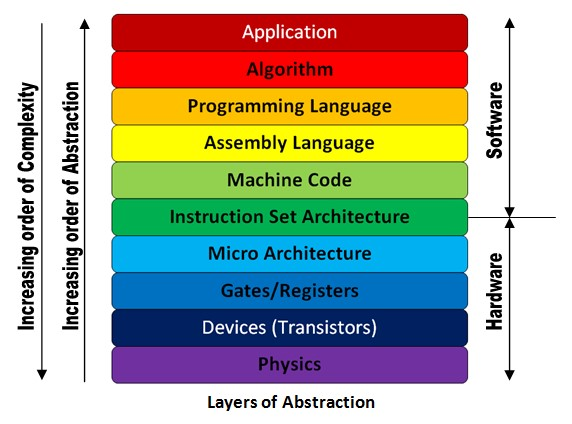
\includegraphics[width=0.95\linewidth]{%
      Graphics/Abstract-Classical-Computing-Stack.jpg}
    
    Image from StackExchange \url{https://electronics.stackexchange.com/q/353915}

  
    \column[T]{0.35\linewidth}
    \begin{block}{Outside-in}
      \begin{enumerate}
      \item Applications
      \item Physical foundations
      \item Building between the extremes
      \end{enumerate}
    \end{block}
  \end{columns}
\end{frame}
